\chapter{Lattice Gauge Theory} \label{chap::lattice_gauge_thy}

%%%%%%%%%%%%%%%%%%%%%%%%%%%%%%%%%%%%%%%%%%%%%%%%%%%%%%%%%
%%%%%%%%%%%%%%%%%%%%%%%%%%%%%%%%%%%%%%%%%%%%%%%%%%%%%%%%%
%%%%%%%%%%%%%%%%%%%%%%%%%%%%%%%%%%%%%%%%%%%%%%%%%%%%%%%%%
%lattice
The properties of hadrons constructed from strongly interacting quarks and gluons should be calculable within the relevant gauge field theory, Quantum Chromodynamics (QCD). At the energy scale of hadrons, QCD does not have a small coupling constant and must be treated non-perturbatively. The tool we will use to achieve this is lattice QCD, in which the field theory is discretized on a finite grid of Euclidean space-time points, and where we can compute correlation functions as an average over a finite but large number of possible gauge-field configurations. In this chapter we will explore the gauge theory, QCD, and show how one can map the theory onto a discrete set of space-time points which when coupled with an analytic continuation of time allows for the calculation of observables. 

%%%%%%%%%%%%%%%%%%%%%%%%%%%%%%%%%%%%%%%%%%%%%%%%%%%%%%%%%
%%%%%%%%%%%%%%%%%%%%%%%%%%%%%%%%%%%%%%%%%%%%%%%%%%%%%%%%%
%%%%%%%%%%%%%%%%%%%%%%%%%%%%%%%%%%%%%%%%%%%%%%%%%%%%%%%%%

\section{The Path Integral } \label{QCD::path_integral}
The functional integral formalism underpins modern understanding of quantum field theory. It was originally introduced by Feynman in the context of quantum mechanics later gaining widespread use in quantum field theory. We will proceed to sketch the basics of the Feynman path integral in this section using simple examples from ordinary quantum mechanics. 

Throughout this section we will follow the traditional \emph{physics style} mathematics in which we use words like ``function" and ``eigenstate" improperly, exchange the order of limits, and commute integrals without consideration for the deeper mathematical issues in the interest of skipping technical details that would obscure the physical understanding. We will work in natural units in which $\hbar = c = 1$. 

%%%%%%%%%%%%%%%%%%%%%%%%%%%%%%%%%%%%%%%%%%%%%%%%%%%%%%%%%
%%%%%%%%%%%%%%%%%%%%%%%%%%%%%%%%%%%%%%%%%%%%%%%%%%%%%%%%%
%%%%%%%%%%%%%%%%%%%%%%%%%%%%%%%%%%%%%%%%%%%%%%%%%%%%%%%%%

\subsection{Feynman Path Integral} 
In quantum mechanics the fundamental objects of interest are probability amplitudes, represented by complex numbers, which describe the physical properties of the particle we seek to measure (position, momentum, spin-projection, etc.). 

We will proceed to illustrate path integral techniques by exploring the probability amplitude for a particle to move from some point $y$ to some point $x$ within an interval of time, $t$ in one dimension. This amplitude is 

\begin{equation*}
A(x,y;t) = \langle x | \mathbf{U}(t) | y \rangle ,
\end{equation*}

where $|y\rangle$ is an eigenstate of the position operator, $\mathbf{U}(t) = e^{-i\mathbf{H}t}$ is the time evolution operator, and $\mathbf{H}$ represents the Hamiltonian which for a free particle is 
\begin{equation*}
\mathbf{H}=\mathbf{H_0} =  \frac{\mathbf{P}^2}{2m},
\end{equation*}
where $\mathbf{P}$ is the momentum operator. Throughout this chapter we make use of bold symbols to represent operators.

 Inserting a completeness relation for momentum states the amplitude becomes 
\begin{align*}
A(x,y;t) &= \int dp \langle x |p \rangle \langle p | y \rangle e^{-i\frac{p^2}{2m}t} \\
&=\int \frac{dp}{2\pi}e^{-i\frac{p^2}{2m}t} e^{ip(x-y)} \\
&= e^{i \frac{m}{2t}(x-y)^2} \int \frac{dp}{2\pi} e^{-i\left(\sqrt{\frac{t}{2m}}p + \sqrt{\frac{m}{2t}}(x-y)\right)^2} \\
&= \sqrt{\frac{2m}{t}}\frac{1}{2\pi}e^{i \frac{m}{2t}(x-y)^2}\int dp e^{-ip^2} \\
&= \sqrt{\frac{m}{2\pi it}}e^{i \frac{m}{2t}(x-y)^2}
\end{align*}
where the last integral can be performed in the complex plane using a contour. If move to a more complicated problem, one in which the particle moves in a local potential $V(x)$ then the Hamiltonian and thus the time evolution operator become more complicated, 
\begin{equation*}
\mathbf{H} = \mathbf{H_0} + V(\mathbf{x}) \qquad \mathbf{U}(t) = e^{-i \mathbf{H} t}.
\end{equation*}

For small times the time evolution operator can be approximated by 
\begin{equation*}
\mathbf{U}(\epsilon) = e^{-iV(\mathbf{x})\epsilon/2}e^{-i\mathbf{H_0}\epsilon}e^{-iV(\mathbf{x}) \epsilon/2} + \mathcal{O}(\epsilon^3)
\end{equation*}
from which it follows that the matrix elements are 
\begin{equation*}
\langle x | \mathbf{U}(\epsilon) | y \rangle = \sqrt{\frac{m}{2\pi i\epsilon}}e^{i \frac{m}{2\epsilon}(x-y)^2 -i \frac{\epsilon}{2}\left[ V(x) + V(y) \right]}  + \mathcal{O}(\epsilon^3).
\end{equation*}

This is sufficient information to construct the path integral. Let us imagine splitting the time interval into $N$ segments, $\epsilon = t/N$, and inserting $N-1$ complete sets of position eigenstates, one between each small evolution, then we may approximate the matrix element as 

\begin{align*}
\langle x | \mathbf{U}(t) | y \rangle &= \lim_{N\to \infty} \int dx_1 \ldots dx_{N-1} \langle x | \mathbf{U}(\epsilon) | x_1 \rangle \ldots \langle x_{N-1} | \mathbf{U}(\epsilon) | y \rangle  \\
&= \lim_{N\to \infty}\left(\frac{m}{2\pi i\epsilon}\right)^{\frac{N}{2}}e^{ i \frac{m}{2\epsilon} \left( [x-x_1]^2 + \ldots + [x_{N-1} -y]^2 \right) -i\epsilon \left( \frac{V(x)}{2} + V(x_1) + \ldots + V(x_{N-1}) + \frac{V(y)}{2}\right)}.
\end{align*}

The exponentiated quantity, in the limit of $N \to \infty$ is the action 
\begin{equation*}
S = \int_0^t dt' \left[ \frac{m}{2} \dot{x}^2 - V(x) \right] 
\end{equation*}
and so we can rewrite the amplitude as 
\begin{equation}
\langle x | \mathbf{U}(t) | y \rangle = \int D[x] e^{iS}, \qquad D[x] = \lim_{N\to \infty}\left(\frac{m}{2\pi i\epsilon}\right)^{\frac{N}{2}} dx_1 \ldots dx_{N-1}. \label{QCD::qm_mink_path_integral}
\end{equation}

Equation \ref{QCD::qm_mink_path_integral} defines the path integral, it is a weighted sum over classical paths where we have removed the ordinary quantum mechanical operators in favor of an infinite dimensional integral, a \emph{functional integral}. 

On first inspection it is somewhat difficult to ascribe meaning to the functional integral,  the integrand is complex and wildly oscillating, further it is an integral over a space of functions. Conversely writing amplitudes in this form allows for efficient and compact derivations, it is a corner stone of quantum field theory. We will see next that the introduction of imaginary time, \emph{Euclidean time}, allows for a more intuitive interpretation of the functional integral and further immediately lends itself to explicit numeric calculation. 

%%%%%%%%%%%%%%%%%%%%%%%%%%%%%%%%%%%%%%%%%%%%%%%%%%%%%%%%%
%%%%%%%%%%%%%%%%%%%%%%%%%%%%%%%%%%%%%%%%%%%%%%%%%%%%%%%%%
%%%%%%%%%%%%%%%%%%%%%%%%%%%%%%%%%%%%%%%%%%%%%%%%%%%%%%%%%

\subsection{Euclidean Path Integral } \label{QCD::Euclidean_path_integral} 

Details on the analytic continuation of time into the complex plane can be found in any standard textbook on quantum field theory. Practically the continuation is achieved by taking $t = -i\tau$, $\tau > 0$ and replacing the time evolution operator by $\mathbf{U}(-i\tau) = e^{-i\mathbf{H}(-i\tau)} = e^{-\mathbf{H}\tau}$.

Repeating the same set of steps we see that the \emph{Euclidean} amplitude is 

 \begin{align*}
\langle x | \mathbf{U}(-i\tau) | y \rangle &= \lim_{N\to \infty} \int dx_1 \ldots dx_{N-1} \langle x | \mathbf{U}(-i\epsilon) | x_1 \rangle \ldots \langle x_{N-1} | \mathbf{U}(-i\epsilon) | y \rangle  \\
&= \lim_{N\to \infty}\left(\frac{m}{2\pi \epsilon}\right)^{\frac{N}{2}}e^{ - \frac{m}{2\epsilon} \left( [x-x_1]^2 + \ldots + [x_{N-1} -y]^2 \right) - \epsilon \left( \frac{V(x)}{2} + V(x_1) + \ldots + V(x_{N-1}) + \frac{V(y)}{2}\right)} \\
&= \int D[x_E] e^{-S_E}.
\end{align*}

\begin{equation*}
D[x_E] = \lim_{N\to \infty} \left(\frac{m}{2\pi \epsilon}\right)^{\frac{N}{2}} dx_1 \ldots dx_{N-1}. 
\end{equation*}

In the interest of notational brevity we will not distinguish between Euclidean and ordinary time differentials $D[x]$, this information is provided by the presence (absence) of $i$ in expressions containing the exponentiation of the action.

We skip the technical details but noted that the full functional integral is defined as a limit in which the discretization is removed. Prior to taking this limit the above formula actually defines a discretization of the amplitude on a Euclidean time lattice with spacing $\epsilon$. 

The Euclidean time evolution operator, the \emph{transfer matrix}, which shifts by one  $\epsilon$-sized unit of time in $\tau$ is 
\begin{equation*}
\mathbf{T}= e^{-V(\mathbf{x})\epsilon/2}e^{-\mathbf{H_0}\epsilon}e^{-V(\mathbf{x}) \epsilon/2} . 
\end{equation*}
The time evolution operator has matrix elements 
\begin{equation*}
\langle x | \mathbf{T} | y \rangle = \sqrt{\frac{m}{2\pi \epsilon}}e^{- \frac{m}{2\epsilon}(x-y)^2 - \frac{\epsilon}{2}\left[ V(x) + V(y) \right]}  
\end{equation*} 
and is related to the Hamiltonian of the discretized theory by $\mathbf{T} = e^{-\epsilon \mathbf{H}}$ which in the limit $\epsilon \to 0$ becomes equal to the Hamiltonian of the continuous theory. 

Generically when one discretizes the theory we consider a hyper-toroid in which there are periodic boundary conditions (e.g. $x(0) = x(L_t))$ where $L_t$ is for example the length in the temporal direction.  The continuum infinite volume theory then also involves taking the length of the time direction to be infinitely large.  

In field theory the amplitudes we work with will be given by \emph{correlation functions} which describe the degree to which measurements of the field at different space-time points acre correlated. For this simplest example we could imagine asking how the measurement of the position of the particle is correlated at different times. Generically we write such a correlation function as 
\begin{equation*}
\trace{ x(t_1) \ldots x(t_n) }
\end{equation*} 
where here the trace is over the complete Hilbert space of the theory. Recalling the time evolution of an operator, $A$, is $A(t) = e^{iHt}A(0)e^{-iHt}$ we see the above equation becomes 
\begin{equation*}
\trace{ x(t_1) \ldots x(t_n) } = \trace{ e^{iHt_1}\mathbf{x}e^{-iH(t_1 -t_2)} \mathbf{x}\ldots \mathbf{x} e^{-iH(t_{n-1} - t_n)} \mathbf{x} e^{-iHt_n }}
\end{equation*} 
where $0 < t_i < L_t$.  Assuming the correlation function can be continued to Euclidean time this becomes  
\begin{equation*}
\trace{ x(\tau_1) \ldots x(\tau_n) } = \trace{ e^{H\tau}\mathbf{x}e^{-H(\tau_1 -\tau_2)} \mathbf{x}\ldots \mathbf{x} e^{-H(\tau_{n-1} - \tau_n)} \mathbf{x} e^{-H\tau_n }}
\end{equation*} 

If we are only interested in the ground state of the theory we can consider the limit $L_t \to \infty$. Defining the generating functional (partition function) 

\begin{equation*}
Z(L_t) = \int D[x] e^{-S_E} = \trace{e^{-HL_t}} = \sum_{\estate{n}}e^{-E_{\estate{n}}L_t},
\end{equation*}

we see that for $t_i > t_{i+1}$
\begin{align*}
&\lim_{L_t\to\infty} \frac{1}{Z(L_t)}\trace{ e^{H\tau}\mathbf{x}e^{-H(\tau_1 -\tau_2)} \mathbf{x}\ldots \mathbf{x} e^{-H(\tau_{n-1} - \tau_n)} \mathbf{x} e^{-H\tau_n }} \\
&= \lim_{L_t\to\infty} \frac{1}{Z(L_t)}\int dx \; \langle x | e^{H\tau}\mathbf{x}e^{-H(\tau_1 -\tau_2)} \mathbf{x}\ldots \mathbf{x} e^{-H(\tau_{n-1} - \tau_n)} \mathbf{x} e^{-H\tau_n } | x \rangle \\
&= \lim_{L_t\to\infty} \frac{1}{Z(L_t)}\int D[x] \;\; x(\tau_1)\ldots x(\tau_n)e^{-S_E}
\end{align*}
where it is understood that the integral over time in the action runs from $0$ to $L_t$ and the paths we integrate over are periodic under shifts by $L_t$ ($x(t) = x(t + L_t)$). Here we have used $\trace{\mathbf{A}} = \int dx \langle x | \mathbf{A} | x \rangle $. 

Denoting the eigenstates of the Hamiltonian as $|\estate{n_0}\rangle, |\estate{n_0}\rangle, \ldots $ where the states are ordered such that $E_{\estate{n_0}} < E_{\estate{n_1}} < \ldots$ we have finally arrived at the connection between the path integral and quantum mechanical amplitudes which for ground states takes the form 

\begin{equation*}
\langle \estate{n_0} | \mathbf{A} | \estate{n_0} \rangle = \lim_{L_t\to\infty} \frac{1}{Z(L_t)}\int D[x] A e^{-S}
\end{equation*}

where for this simple system we consider $\mathbf{A}$ is some composite operator of the field, $x$, located a different points in time $\tau_i$, for example: 

\begin{equation*}
\langle \estate{n_0} | \mathbf{x}(\tau_1)\ldots \mathbf{x}(\tau_n) | \estate{n_0} \rangle = \lim_{L_t\to\infty} \frac{1}{Z(L_t)}\int D[x] \;\; x(\tau_1)\ldots x(\tau_n)e^{-S_E}.
\end{equation*}

%%%%%%%%%%%%%%%%%%%%%%%%%%%%%%%%%%%%%%%%%%%%%%%%%%%%%%%%%
%%%%%%%%%%%%%%%%%%%%%%%%%%%%%%%%%%%%%%%%%%%%%%%%%%%%%%%%%
%%%%%%%%%%%%%%%%%%%%%%%%%%%%%%%%%%%%%%%%%%%%%%%%%%%%%%%%%


\section{Lattice Discretization} \label{QCD::lattice_discretization} 
While the path integral is formally defined in the infinite volume continuum limit practical applications tend to work in the limit of both finite volume and with a finite discretization scale. Such simulations, performed on a finite grid in a finite volume, may not necessarily respect the full set of symmetries present in the continuum infinite volume theory. Here we consider some implications, arising from a lattice discretization, using a simple two-dimensional model in order to build intuition. 

Forgetting for a moment that we actually live in three spatial dimensions let us consider a two spatial dimensional world and consider the implication of a grid-like discretization on angular momentum wave functions. In order to fully simplify the example we will also consider a discretization which has the same symmetries as the boundary. More simply let us just consider a square grid of side $L$ with a discretization $a$ defined by $L = Na$ where $N$ is the number of lattice sites along each side of the square as in \figref{fig::2Dlattice}. 

\begin{figure}[htbp]
\centering
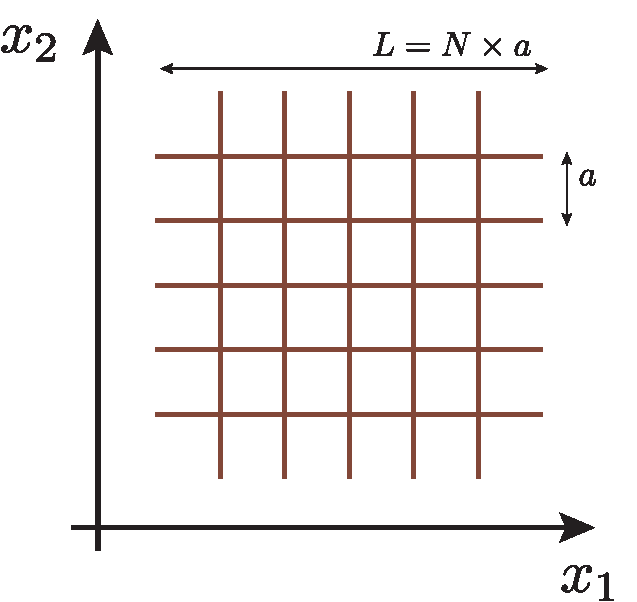
\includegraphics[width=0.5\linewidth]{figures/2DLattice/2dLattice.pdf}
\caption{ A two dimensional lattice discretization. \label{fig::2Dlattice}}
\end{figure}

Here we attempt to build some intuition related to the practical implications arising when simulating on a finite mesh in a finite volume by considering the effect of lattice discretization on angular wave functions. In cartesian coordinates the two dimensional Laplacian operator is defined as $\nabla^2 = \frac{d^2}{dx_1^2} + \frac{d^2}{dx_2^2}$. In polar coordinates the Laplacian takes the form $\nabla^2 = \frac{1}{r}\frac{d}{dr} r \frac{d}{dr} + \frac{1}{r^2} \frac{d^2}{d\phi^2}$. The Schrodinger Equation for a free particle takes the form 

\begin{equation*}
-\frac{1}{2m}\nabla^2 \psi(r,\phi) = E \psi(r,\phi).
\end{equation*}
The wave function, $\psi(r,\phi)$, is separable, it can be written as $\psi(r,\phi) = R(r)\Phi(\phi)$ where $\Phi(\phi) \sim e^{im\phi}$. Provided we are in a continuous infinite volume the angular wave functions can be indexed by the value $m$, an integer.  

If however we think about a system such as the one depicted in \figref{fig::2Dlattice} we immediately realize that the grid is only invariant under rotations by multiples of $\pi/2$. In the same vein we can no longer classify our angular wave functions by an integer, $m$. This is to say that the operator which rotates space by some infinitesimal amount does not commute with the lattice discretized Hamiltonian and thus $m$ is no longer a good quantum number. Rather we are left with the symmetry group corresponding to the four possible rotations by $\pi/2$ and the four possible reflections.

\begin{figure}[htbp]
\centering
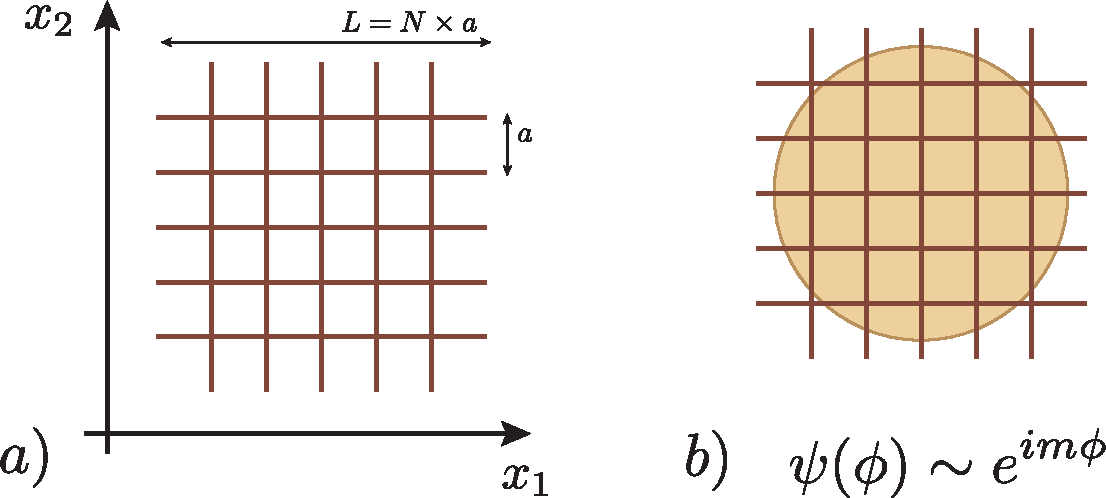
\includegraphics[width=0.7\linewidth]{figures/2DLattice/2dLatticeWavefuncs.pdf}
\caption{ A two dimensional lattice discretization. \label{fig::2DlatticeWavefuncs}}
\end{figure}

One readily identifiable consequence of the reduced symmetry is the realization that under rotations by $\pi/2$ we have lost the ability to distinguish $m=0$ from $m=4$, angular wave functions for the two values both being invariant under the allowed rotations. We will see later in the manuscript that such arguments also apply to the cubic discretization we will use in this calculation. Particles transforming like spin $J$ in the continuum are instead labeled by the irreducible symmetry groups of the box, multiple values of $J$ being present in any one symmetry group.  

The finite volume nature of the calculation also necessitates the use of a box which is large enough to readily accommodate the particle content of the theory. For example, if we consider the quantum mechanics of our free particle, we expect it to have some characteristic length scale. In ordinary quantum mechanics we might estimate this radial scale as 
\begin{equation*}
\langle r \rangle  = \int r drd\phi \; \psi^*(r,\phi) \psi(r,\phi) r.
\end{equation*}  

Another estimate might be the Compton wavelength of the particle, $\lambda = \frac{1}{m}$. In both cases we should require that the box is large enough such that the particle does not interact with the boundary. A toy example of this can be seen in \figref{fig::2DlatticeCompton} where we consider how the boundary might effect the particle. Simply put we require that the box be large enough to accommodate the particle of interest. 


\begin{figure}[htbp]
\centering
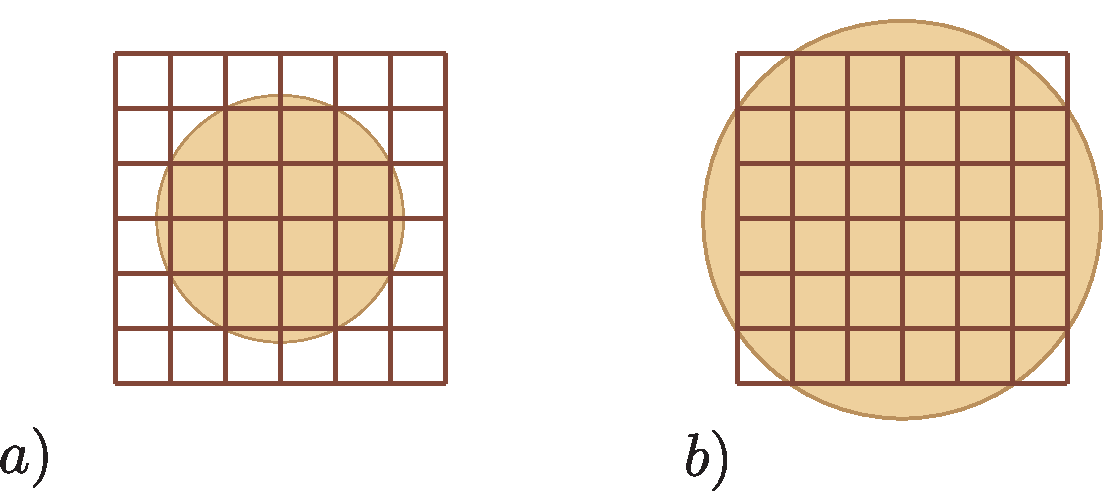
\includegraphics[width=0.7\linewidth]{figures/2DLattice/2dLatticeCompton.pdf}
\caption{ A two dimensional lattice discretization. \label{fig::2DlatticeCompton}}
\end{figure}



%%%%%%%%%%%%%%%%%%%%%%%%%%%%%%%%%%%%%%%%%%%%%%%%%%%%%%%%%
%%%%%%%%%%%%%%%%%%%%%%%%%%%%%%%%%%%%%%%%%%%%%%%%%%%%%%%%%
%%%%%%%%%%%%%%%%%%%%%%%%%%%%%%%%%%%%%%%%%%%%%%%%%%%%%%%%%


\section{QCD on a lattice} \label{QCD::lattice} 


%%%%%%%%%%%%%%%%%%%%%%%%%%%%%%%%%%%%%%%%%%%%%%%%%%%%%%%%%
%%%%%%%%%%%%%%%%%%%%%%%%%%%%%%%%%%%%%%%%%%%%%%%%%%%%%%%%%
%%%%%%%%%%%%%%%%%%%%%%%%%%%%%%%%%%%%%%%%%%%%%%%%%%%%%%%%%

\subsection{QCD generating functional \label{QCD::generating_functional}}
Having introduced the path integral formalism in the context of ordinary quantum mechanics we now turn to the generating functional of QCD. As previously mentioned at the energy scale of hadrons the coupling of QCD is large and the standard perturbative expansions of quantum field theory do not converge.  

In order to circumvent this difficulty we will proceed to directly evaluate the path integral by numeric simulation over a large but finite number of ``paths''. Here the fundamental degrees of freedom are the quark and gluon fields and the path integral corresponds to integrating over all values of these fields at each point in space-time.

 In order to frame the discussion we now introduce the QCD generating functional, it may be written as:

\begin{equation}
\mathcal{Z} = \int D[\psi \; \bar{\psi} \;A] e^{-S[\psi \;\bar{\psi}\;A]}.
\end{equation} 

The action, $S$, is the four dimensional integral over space-time of the Lagrange density, 
\begin{equation*}
S = \int d^4x_E \; \mathcal{L}(x)
\end{equation*}
where the Lagrange density, $\mathcal{L}(x)$ is 
\begin{equation}
\bar{\psi}\left[i \gamma_\mu d_\mu - m\right]\psi - g \gamma_\mu A_\mu^a\bar{\psi}t^a\psi - \frac{1}{4}G_{\mu\nu}^aG_{\mu\nu}^a.
\end{equation}

The quark fields, denoted by $\psi^\alpha_i(x)$,  are color-spinor fields which are a functions of the space-time coordinate, $x$, with $SU(3)$ color index $i=1,2,3$ and Dirac spinor index $\alpha=0,1,2,3$. We have suppressed the flavor index, for the main portion of this manuscript we will consider an unphysical version of QCD in which we have three degenerate quark flavors all tuned to approximately the strange quark mass. The quark fields themselves transform locally under $SU(3)$ color gauge rotations while the Lagrange density is a \emph{gauge invariant} scalar density. 

The gluon fields, $A_u^a$, transform as Lorentz vectors and have a color index $a=1-8$ corresponding to the adjoint representation of $SU(3)$ while the $t^a$ are the generators of the gauge group, one possible basis being the Gell-Mann matrices. 

The $\gamma_\mu$ are Dirac matrices and in \emph{Euclidean} space obey the anti-commutation relation $\{\gamma_\mu,\gamma_\nu\} \equiv \gamma_\mu\gamma_\nu - \gamma_\nu,\gamma_\mu = 2\delta_{\mu\nu}\mathbf{1}$.  $G_{\mu\nu}^a$ is the field strength tensor for the chromo-magnetic and chromo-electric fields, it is defined as 
\begin{equation*}
G_{\mu\nu}^a = \partial_\mu A_\nu^a - \partial_\nu A_\mu^a - gf^{abc}A^b_\mu A^c_\nu,
\end{equation*}
where $g$ is the coupling and $f^{abc}$ are the structure constants which re-express the Lie brackets of pairs of generators as a linear combination of generators from the same set (i.e. $\left[t^a,t^b\right] = f^{abc}t^c$).

%%%%%%%%%%%%%%%%%%%%%%%%%%%%%%%%%%%%%%%%%%%%%%%%%%%%%%%%%
%%%%%%%%%%%%%%%%%%%%%%%%%%%%%%%%%%%%%%%%%%%%%%%%%%%%%%%%%
%%%%%%%%%%%%%%%%%%%%%%%%%%%%%%%%%%%%%%%%%%%%%%%%%%%%%%%%%

\subsection{Correlation Functions on a continuous Euclidean Toroid} \label{QCD::correlators}

The fundamental objects we will be working with are \emph{correlation functions} which in some loose sense measures the degree to which a perturbation at some space-time point, $x$, propagates to some other space-time point y.  A simple intuitive example from macroscopic physics is the ripples that one finds in a still pond after tossing a stone into the middle. The ripples have some characteristic velocity with which they expand, telling us where to find them in time, while their amplitude decreases with radial distance which tells us something about how they expand. 

In general we will be interested in calculating \emph{correlation functions} of colorless combinations of quark and gluon fields located at different points in space-time on a Euclidean lattice. As a primer we can first think about QCD with one spatial dimension and one temporal direction in continuous space-time, such a theory is commonly referred to as a $1+1$ dimensional field theory. A visualization of the space-time of such a theory is depicted in \figref{fig::QCD_1p1_lattice}. 

\begin{figure}[htbp]
\centering
\includegraphics[width=0.8\linewidth]{figures/lattice_toroid/lattice_toroid.pdf}
\caption{ A $1+1$ dimensional toroid. \label{fig::QCD_1p1_lattice}}
\end{figure}

Surfaces of constant time are marked at $t=t_1$ and $t=t_2$. Letting $\mathcal{O}(t)$ represent some generic color singlet operator composed out of quark and gluon fields a general object of interest we can study is the vacuum to vacuum expectation value 
\begin{equation*}
\langle 0 | \mathcal{O}(t_2) \mathcal{O}^\dagger(t_1) | 0 \rangle 
\end{equation*}
which describes the amplitude to create a particle at $t=t_1$ and later annihilate the particle at $t=t_2$, where the dagger symbol denotes Hermitian conjugation. In a manner similar to that derived in Section~\ref{QCD::Euclidean_path_integral} this amplitude is given by 

\begin{equation*}
\langle 0 | \mathcal{O}(t_2) \mathcal{O}^\dagger(t_1) | 0 \rangle  = \lim_{L_t \to \infty} \frac{1}{\mathcal{Z}} \int D[\psi \; \bar{\psi} \;A] \;  \mathcal{O}(t_2) \mathcal{O}^\dagger(t_1) \; e^{-S[\psi \;\bar{\psi}\;A]}.
\end{equation*} 

Formally the correlation function is obtained only in the limit where the temporal length of the toroid is infinitely large. This is readily understood on the basis of \figref{fig::QCD_1p1_lattice_finit_T}, we see that there is a ``short path'' (red) from $t_1$ to $t_2$ as well as a longer path (blue) corresponding to so called ``backwards propagation'' in which the particle is created at $t_1$ and travels backwards in time finally annihilating at $t_2$. There are also several images in which the particle travels around the length of the toroid several times before annihilating. 

\begin{figure}[htbp]
\centering
\includegraphics[width=0.8\linewidth]{figures/lattice_toroid_finit_T/lattice_toroid_finit_T.pdf}
\caption{ A $1+1$ dimensional toroid and finit temperature effects. \label{fig::QCD_1p1_lattice_finit_T}}
\end{figure}


These corrections, which disappear in the limit that the temporal length of the toroid becomes infinitely large, are referred to as \emph{finite temperature} corrections. For the Euclidean correlation functions we consider the corrections enter with powers of the pre-factor $e^{-E_{\estate{0}}L_t}$ where $E_{\estate{0}}$ is the lightest mode that can propagate and $L_t$ is the temporal length of the toroid. Provided that the temporal length of the toroid is sufficiently large it is a good approximation to simply neglect the existence exponentially damped finite temperature effects. Then up to suppressed finite temperature effects we see that vacuum to vacuum correlation functions are give by 
\begin{equation*}
\langle 0 | \mathcal{O}(t_2) \mathcal{O}^\dagger(t_1) | 0 \rangle  = \frac{1}{\mathcal{Z}} \int D[\psi \; \bar{\psi} \;A] \;  \mathcal{O}(t_2) \mathcal{O}^\dagger(t_1) \; e^{-S[\psi \;\bar{\psi}\;A]}.
\end{equation*} 




%%%%%%%%%%%%%%%%%%%%%%%%%%%%%%%%%%%%%%%%%%%%%%%%%%%%%%%%%
%%%%%%%%%%%%%%%%%%%%%%%%%%%%%%%%%%%%%%%%%%%%%%%%%%%%%%%%%
%%%%%%%%%%%%%%%%%%%%%%%%%%%%%%%%%%%%%%%%%%%%%%%%%%%%%%%%%
\subsection{Correlation Functions on a Euclidean Lattice} \label{QCD::lattice_correlators}

Having reviewed the generating functional and correlation functions in continuous space-time we now turn to the discretization of the path integral onto a Euclidean time lattice. Working in a discrete space-time it is natural to label the nodes of the lattice by a vector of integers, $\vec{n} = [n_x , n_y , n_z , n_t]$. Using $a$ to denote the lattice spacing, the allowed space-time coordinates are $\vec{x}_{\vec{n}} = a\;\vec{n}$. Here we will specialize to a case where the length of the box is the same in all directions, $L_{x}= L_{y} = L_z = L_t = N a = L$, where we have imagined that we have divided each direction into $N$ segments\footnote{Later in the text we will consider QCD on an anisotropic lattice where the discretization along the temporal direction is finer than along the spatial directions.}. 

The continuum quark fields, $\psi^\alpha_i(x)$, reside on the nodes of the lattice. They obey periodic boundary conditions in the spatial direction,  $\psi^\alpha_i(x) = \psi^\alpha_i(x + L)$, and anti-periodic boundary conditions in time. The anti-periodic boundary conditions in time are a consequence of putting fermions on a toroid, the sign must be introduced to make the density matrix positive definite. 

In the continuum theory the gluon fields $A^a_\mu$ appear in the ``parallel transporters'' 
\begin{equation*}
U(x,y) \equiv \mathcal{P}\{e^{ig \int_x^y dz_\mu A^a_\mu(z) t^a }\}
\end{equation*} 
which tell us how to accumulate color phase as we move through space. There is an implied summation on the color index, $a$. Here the symbol $\mathcal{P}$ denotes a path ordering and simply means to compute the exponentiated integral along some specific path from $x$ to $y$. When we discretize the theory the parallel transporters must be anchored at the nodes of the lattice, we call the resulting transporters which take us from one node to its neighbor \emph{gauge links}, they are elements of $SU(3)$ and are defined as: 
\begin{equation*}
U_\mu(x) \equiv U(x,x+\hat{\mu}) =  e^{ig a A^c_\mu(x) t^c }. 
\end{equation*} 
Where a is the lattice spacing along the $\mu$ direction. 

In \figref{fig::QCD_1p1_lattice_fields} we show a toy representation of the discretization of QCD in $1+1$ dimensions. The fermion fields ``live" on the lattice sites while the gluons are contained in the gauge links that connect neighboring sites. The operators $\mathcal{O}$ defined above in Section \ref{QCD::correlators} are constructed out of gauge invariant, color singlet, combinations of the quark fields and gauge links. 

\begin{figure}[htbp]
\centering
\includegraphics[width=0.8\linewidth]{figures/lattice_toroid_fields/lattice_toroid_fields.pdf}
\caption{ A $1+1$ dimensional toroid. When we discretize QCD onto a lattice the quark fields $\psi$ sit on the nodes of the lattice while the gluon fields live along the gauge links in the matrices $U$ which are elements of $SU(3)$. \label{fig::QCD_1p1_lattice_fields}}
\end{figure}

The discretization of the underlying field theory onto a lattice provides us a systematically improvable framework in which we can non-perturbativly evaluate correlation functions in the strongly coupled regime of QCD.

Having reviewed some of the fundamental ideas of quantum field theory we now turn to the technical details of correlator construction, the relationship of correlation functions to matrix elements, and 


..... connect .... 
